\documentclass[12pt]{article}

\usepackage{sbc-template}

\usepackage{graphicx,url}

\usepackage{listings}
\usepackage{color}

\usepackage{booktabs}
\usepackage{multirow}
\usepackage{graphicx}
\usepackage{amsmath}


%\usepackage[brazil]{babel}   
\usepackage[latin1]{inputenc}  

     
\sloppy

\definecolor{mygreen}{rgb}{0,0.6,0}
\definecolor{mygray}{rgb}{0.5,0.5,0.5}
\definecolor{myblue}{rgb}{0,0,0.80}

\graphicspath{{figures/flow/} {figures/automata_comparison/} {figures/lifting_results/} {figures/lifting_time/} {figures/size/}}

\lstdefinestyle{customc}{
  belowcaptionskip=1\baselineskip,
  breaklines=true,
  frame=L,
  xleftmargin=\parindent,
  language=C,
  showstringspaces=false,
  basicstyle=\footnotesize\ttfamily,
  keywordstyle=\bfseries\color{mygreen},
  commentstyle=\itshape\color{purple},
  identifierstyle=\color{myblue},
  stringstyle=\color{orange},
}

\title{MO601 - Project 4 Report \\ Learning Instruction Semantics From Code Generators}

\author{093311 - Alberto Arruda de Oliveira\inst{1}}


\address{Institute of Computing -- University of Campinas
  (UNICAMP)
  \email{\{alberto.oliveira\}@ic.unicamp.br}
}

\begin{document}


\maketitle

\begin{abstract}

Instruction lifting, the process of translating machine instructions into a higher form of intermediate language is crucial for many systems focused on binary analysis and code instrumentation. Hasabnis and Sekar~\cite{Hasabnis2014} proposed the \textit{LISC} (Lifting Instruction Semantics from Code Generators) tool to automatically perform instruction lifting, using information from code generators employed by compilers. In this project, I perform further evaluation of LISC under the scenarios of completeness and performance. The completeness experiments offer a more thorough analysis of LISC's efficiency in properly lifting instructions, given an automata built from different sets of programs. The performance analysis traces the growth of lifting time according to the size of the binary analyzed, as well as a comparison between lifting time considering automata containing different sets of instructions. Moreover, the performance for code lifting is compared in terms of the expected upper bound given in~\cite{Hasabnis2014}

\end{abstract}


\section{Introduction} \label{sec:intro}

Program monitoring and debugging systems, such as Pin~\cite{Pin}, virtualization systems, as well as software security techniques, all rely on binary analysis and instrumentation. The modeling of instruction semantics into a higher level intermediate language is one of the main steps required by tools and algorithms that rely on binary analysis. 
%
%Currently, such modeling is mostly done manually. However, considering the large amount of instruction present on modern architectures (x86, ARM v7), which surpasses the thousands, as well as the complexity of such instruction sets, makes the manual translation a hard and very time consuming process. This, in turn, leads to limited architecture support by popular programs that rely on such models.
%
Hasabnis and Sekar~\cite{Hasabnis2014} propose a system to automatically build the semantic models, based on knowledge that can be obtained from modern compilers such as GCC. Since compilers employ code generators to convert an \textit{Intermediate Language}(IL) into binary instructions, the authors argue that it is reasonable that by learning from such those generators, it is possible to perform the inverse. The main advantages of using this approach, besides its automated nature, is that the resulting code is \textit{architecture neutral}, and the binary lifting relies on compiler code, which is very robust and well tested. Besides the development of the LISC tool, Hasabnis and Sekar~\cite{Hasabnis2014} also proposed a evaluation framework for their tool, which considers areas such as completeness and correctness. Figure~\ref{fig:flow} displays an overview of LISC's flow of execution.

In Project 3, my objective was to test the LISC tool made available by Hasabnis and Sekar~\cite{LISC}, and try to reproduce one of the results in~\cite{Hasabnis2014}. However, as detailed in the report for Project 3, the results chosen (displayed here as Table~\ref{tab:lisc_table}), could not be reproduced, due to issues such as difficulty in correctly extracting the code generator logs for some of the executables used, as well as time constraints. Thus, in this project, one of my objectives was to modify the methodology of~\cite{Hasabnis2014}, and reproduce the results for a different set of automata and binary dumps. Such results are discussed in Section~\ref{sec:completeness}.

In addition to the extension of Project 3, I also performed new experiments to show the performance of LISC, which are discussed in Section~\ref{sec:performance}. Section 6.3 of~\cite{Hasabnis2014} briefly discusses performance, showing a graph to display the automata creation time in function of concrete pair number, and in a single paragraph discusses the binary lifting performance. Here, I give an in depth look of the lifting performance, displaying it in function of binary dump size and instruction number. In my results, I show a clear contradiction with the expected complexity to the binary lifting approach of Hasabnis and Sekar. I observed that the lifting size exhibits quadratic growth with the binary size, while the authors claim such growth should be linear. Additionally, I also discuss the lifting time when different automata are used.

\begin{figure}
\centering
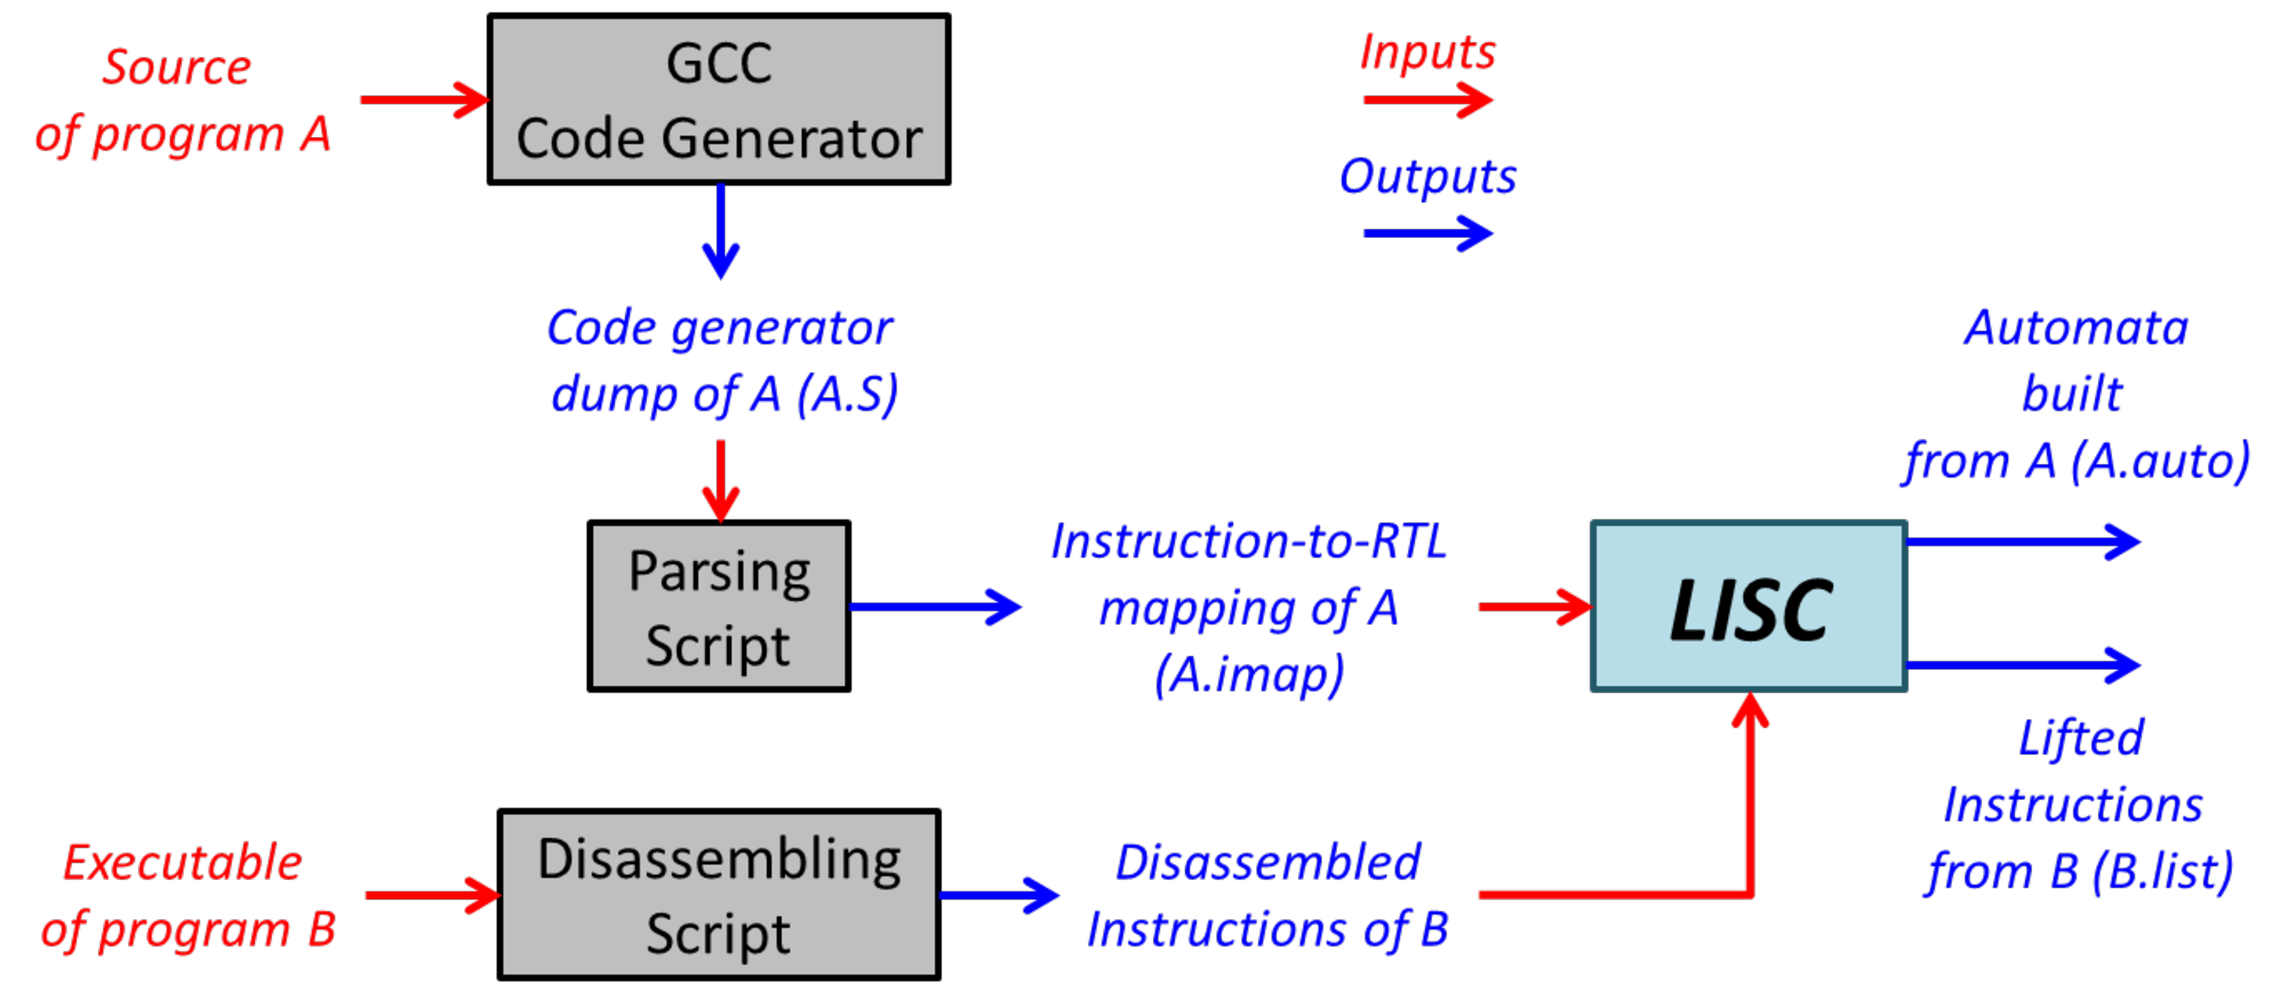
\includegraphics[width=0.5\textwidth]{flow.pdf}%
\caption{Flow of the LISC tool}
\label{fig:flow}
\end{figure}

\section{Completeness Evaluation} \label{sec:completeness}

\begin{table}[ht]
\centering
\caption{Original Results for LISC Completeness}
\label{tab:lisc_table}
\resizebox{0.9\textwidth}{!}{%
\begin{tabular}{@{}l|cc|cc|c@{}}
\toprule
\multirow{2}{*}{\textbf{$P_{train}$}}   & \multicolumn{2}{c|}{\textbf{\% Instructions Lifted}} & \multicolumn{2}{c}{\textbf{LISC (\%)}}                 & \multirow{2}{*}{\textbf{Missing Mnemonics (Absolute)}} \\
                                        & \textbf{Exact Recall}         & \textbf{LISC}        & \textbf{Missing Mnemonics} & \textbf{Missing Operands} &                                                        \\ \midrule
\textbf{openssl-1.0.1f + binutils-2.22} & 63.72                         & 98.46                & 1.05                       & 0.49                      & 464                                                    \\
\textbf{+ffmpeg-2.3.3 (Non opt)}        & 68.21                         & 98.74                & 1.03                       & 0.23                      & 377                                                    \\
\textbf{+glibc-2.21}                    & 68.74                         & 98.80                & 1.01                       & 0.19                      & 346                                                    \\
\textbf{+ffmpeg-2.3.3 (Opt)}            & 69.07                         & 98.89                & 0.88                       & 0.23                      & 303                                                    \\
\textbf{+gstreamer-1.4.5}               & 71.07                         & 99.10                & 0.79                       & 0.11                      & 221                                                    \\
\textbf{+qt-5.4.1}                      & 72.45                         & 99.21                & 0.69                       & 0.09                      & 161                                                    \\
\textbf{+linuxkern-3.19}                & 73.97                         & 99.49                & 0.44                       & 0.07                      & 49                                                     \\
\textbf{+Manual}                        & 74.04                         & 100.00               & 0.00                       & 0.00                      & 0                                                      \\ \bottomrule
\end{tabular}%
}
\end{table}

With Project 3, my objective was to reproduce the completeness experiment described by Hasabnis and Sekar~\cite{Hasabnis2014}, the results of which are presented in table~\ref{tab:lisc_table} here. However, the lack of original instruction mapping files used to generate automata, the unclear nature of the $P_{test}$ set of testing programs, as well as the significantly larger running time of the tool, in comparison to the one reported in their paper, were some of the issues faced in replicating such experiment. Moreover, the tool used to compute the \textit{Exact Recall} measure used as baseline, was lacking in the software package provided by the authors. 

For this Project, I loosely follow the completeness experiment methodology, and perform my own evaluation with the following changes:
\begin{enumerate}
\item A different set of automata used;
\item Binary Lifting was evaluated for each program individually, instead of bundling their instructions;
\end{enumerate}
%
Considering change (2), I use the average lifting accuracy as my evaluation metric. The reasons for evaluating each program separately were twofold: it allowed us to eliminate larger programs, which did not finish lifting in a feasible time; it allows us to model other interesting metrics, such as the relationship between program size and time to perform lifting. Furthermore, I believe that not eliminating duplicate instructions provide a more transparent view of the lifting accuracy, since a instruction that appears as duplicate multiple times, may not be lifted correctly. Around 900 executables were used, with instruction dumps ranging from 6KB to 6MB, summing around 17 million total instructions. Figure~\ref{fig:lifting_accuracy} displays the average lifting accuracy for 7 different automata. As in the original methodology, each automata is complementary to the previous.

\begin{figure}[ht]
\centering
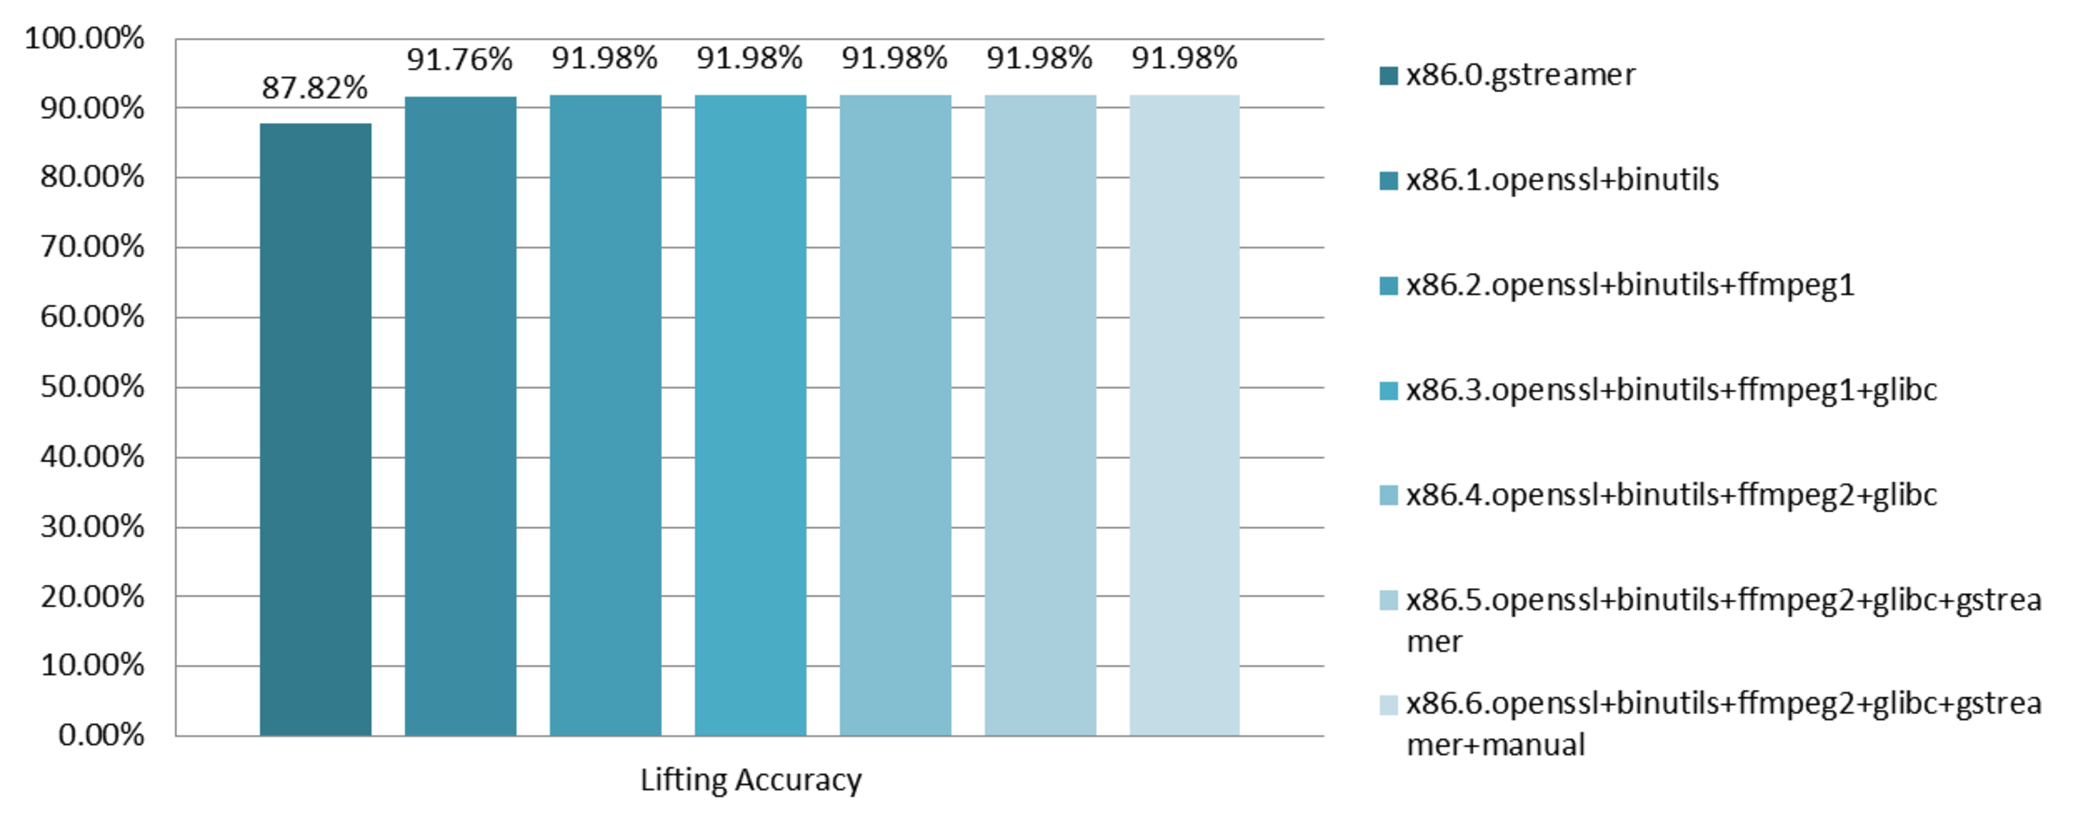
\includegraphics[width=0.7\textwidth]{lifting_results}%
\caption{Average lifting accuracy for different automata}
\label{fig:lifting_accuracy}
\end{figure}

At first glance, the most notable difference is the much lower lifting accuracy in my experiments, in comparison to the original experiment displayed in Table~\ref{tab:lisc_table}. Comparing Table~\ref{tab:lisc_table}'s second row with the second bar of~\ref{fig:lifting_accuracy}, which should yield similar results, we observe a discrepancy of almost 7 percentual points. This result is even more interesting considering that the total amount of instructions in my experiment is far lower than the one in he original experiment (around 17 million for the former and around 40 million for the later). The most distinguished difference between both sets is the presence of duplicate instructions, which might impact the overall result.

It is also interesting to observe that, after the second complementary automata, there was no perceived growth in the average lifting accuracy. This contrasts with the results of the original experiment, whereby each complementary automata exhibited some accuracy gain in comparison to the previous.


\section{Performance Evaluation} \label{sec:performance}

Hasabnis and Sekar~\cite{Hasabnis2014} briefly discuss the performance of their tool, in terms of automata construction time and binary lifting time. A simple graph is provided by the authors displaying the automata construction time in function of the number of instruction-RTL pairs contained in the .imap file. For the lifting time, the authors argue that it took around 8 hours to lift the binaries on Ubuntu (consiting of around 40M unique instructions, a fifth of which was disassembly time.

In this project, I provide a more detailed view of the lifting time, modeling the growth in lifting time in function of executable size, dump size, and instruction number. Adding to that, I also compare the lifting time using different automata, to analyze if the automata size impacts the lifting time.

\subsection{Lifting Performance}\label{subsec:lifting_performance}

\begin{figure}[ht]
\centering
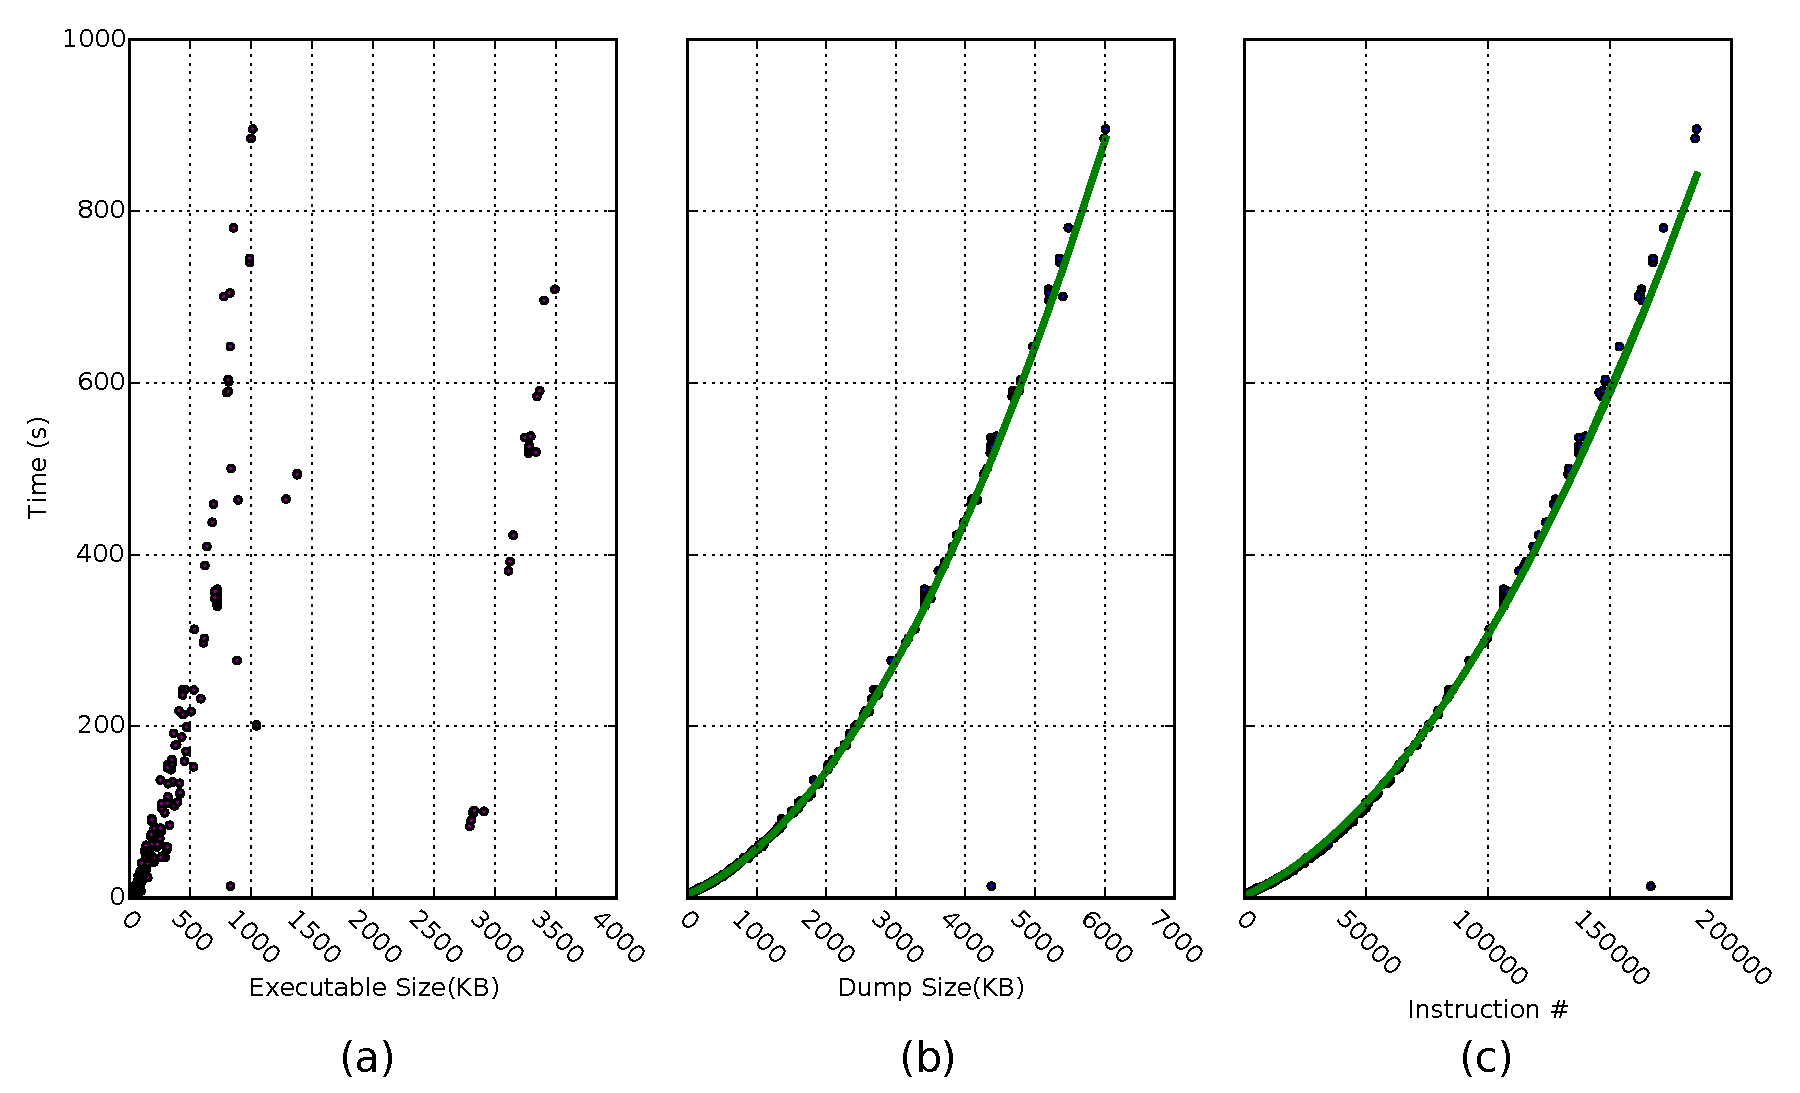
\includegraphics[width=0.7\textwidth]{lifting_time}%
\caption{Lifting time in function of (a) original executable size, (b) dump size after using \textit{objdump}, and (c) total number of instructions, for the x86.3.openssl+binutils+ffmpeg1+glibc automata.}
\label{fig:lifting_time}
\end{figure}

Figure~\ref{fig:lifting_time} displays the lifting time in function of the original executable size, the dump size and the number of instructions in the executable. In Section 4 of~\cite{Hasabnis2014}, the authors describe a Dynamic programming algorithm to lift binaries, with $O(n)$ complexity, $n$ being some measure of the dumped binary size. Their performance discussion in Section 6.3 also describes the lifting time increasing roughly linearly with dump size. However, Figure~\ref{fig:lifting_time} shows a clear contradiction with this assertion, as the time clearly grows in quadratic fashion. In fact, the growth in lifting time made it unfeasible to lift binaries bigger than 9MB, thus resulting in the requirement to limit the size of the used binaries.

The reason for such clear contradiction might be either a mistake in reporting the time by the authors, or the parameter $k$ described in Section 4 of their paper. According to the authors, this parameter is a property of the machine description used in the compiler. However, I did not find any way to modify such parameter. Moreover, I believe the performance evaluation described by the authors is strongly flawed. They argue a lack of space for showing the performance in binary lifting, however they show the automata creation time graph. However, the automata creation time is negligible in comparison to the binary lifting time, and its graph could have easily been skipped in favor of the later. 

The vast majority of the almost 900 binaries utilized clearly follow the quadratic trend shown in Figure~\ref{fig:lifting_time}.b and~\ref{fig:lifting_time}.c. One outlier, however, is \textit{ldconfig}. According to Linux's man page, \textit{ldconfig} is responsible for configuring dynamic linker run-time bindings. \textit{ldconfig} also has two other interesting characteristics, in comparison to other dumped binaries: it is one of the smallest executables to result in a rather big dump (8.2KB executable resulting in a 4.2MB dump), and also had, for all automata, a very low lifting accuracy. For reference, as per the graph displayed in Figure~\ref{fig:lifting_accuracy}, while the average lifting accuracy for the biggest automata (\textit{x86.6}) was 91.98\%, the lifting accuracy for \textit{ldconfig} as a measly 0.1\%. For reference, the second lowest lifting accuracy for the same automata was 77.4\%. Further analysis of some intrinsic characteristics of \textit{ldconfig}, such as the number of \textit{nops}, and total unique instructions lead to no conclusion a to why its lifting accuracy was so low.

\begin{figure}[ht]
\centering
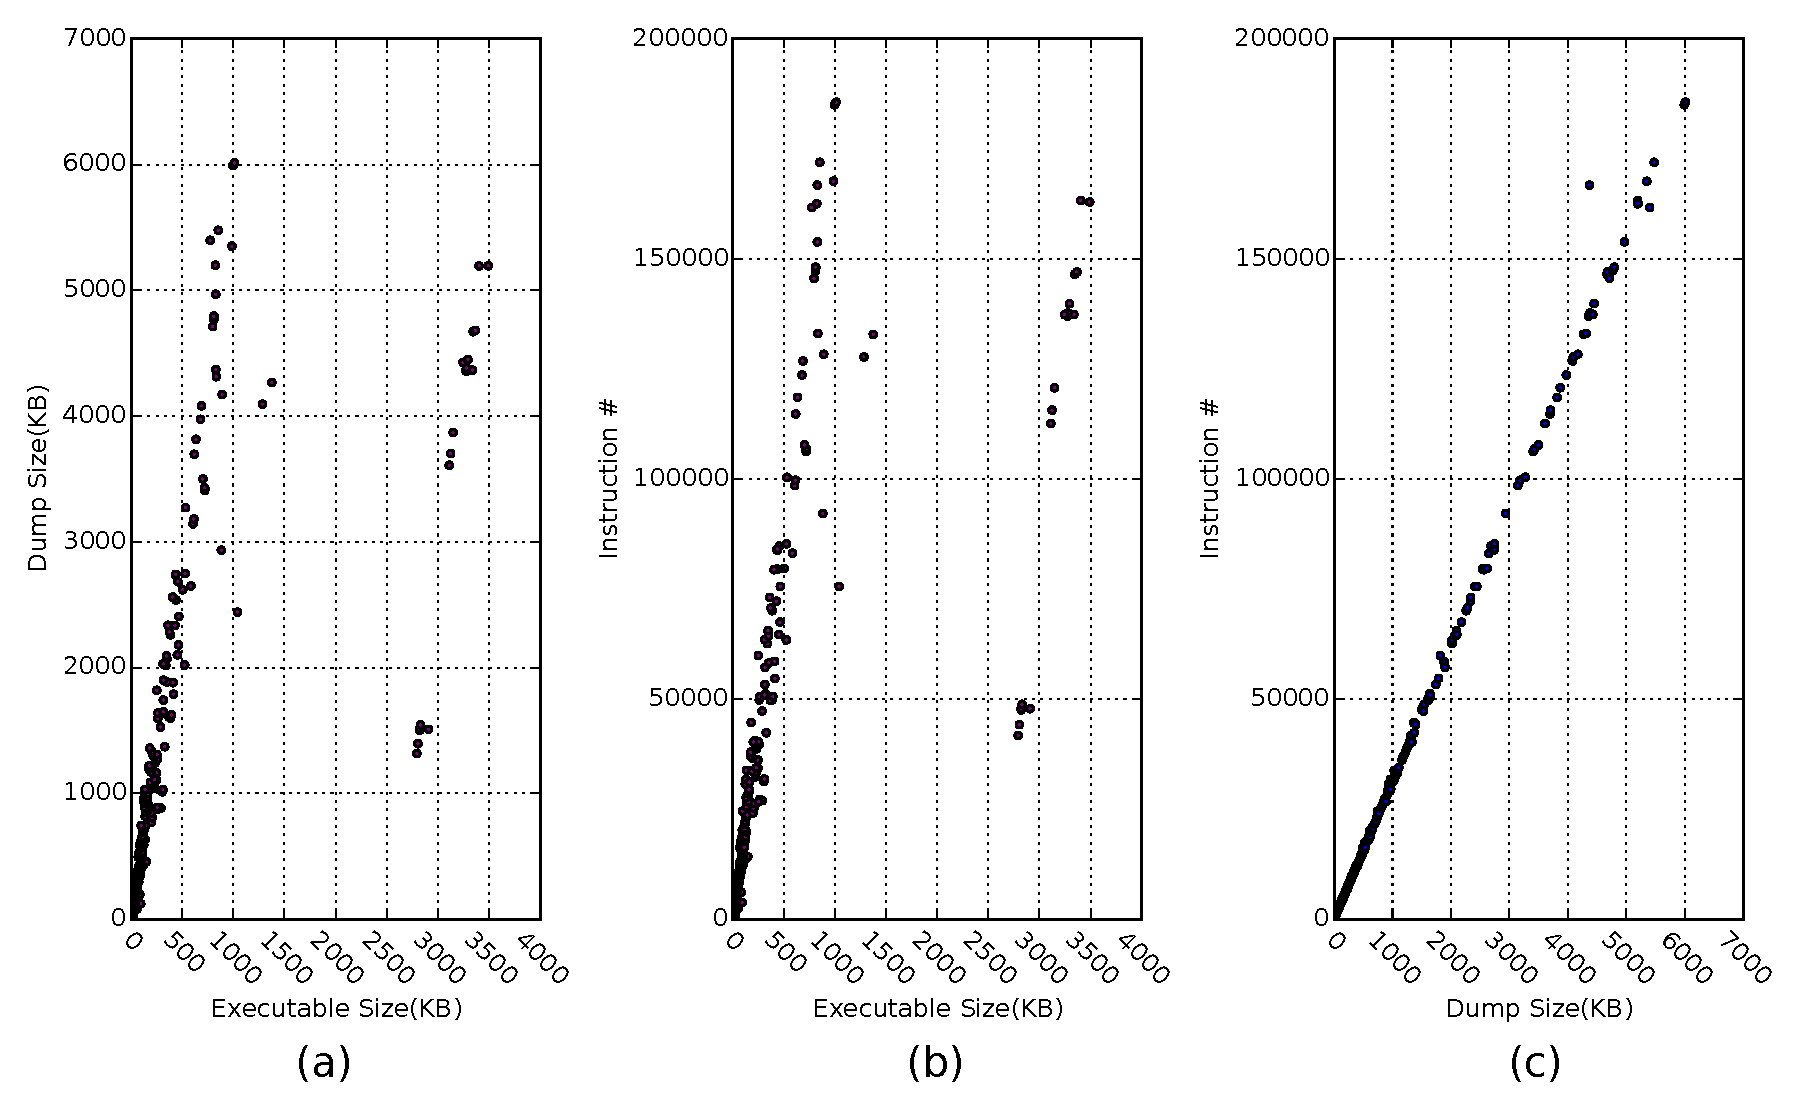
\includegraphics[width=0.7\textwidth]{size}%
\caption{(a) Dump size and (b) Instruction number in function of Executable size, and (c) Instruction number in function of Dump size, for the openssl+binutils+ffmpeg1+glibc automata. }
\label{fig:size}
\end{figure}

Additionally to the time analysis, Figure~\ref{fig:size} provides an overview of the size relationships between the original executables and their dumps. In general, the trend followed by most executables is that the bigger their size, the bigger their dump is. However, as per the graph, there are at least two size trends, one from 0KB to around 15MB, and the other from around 2.7MB to 3.5MB. This may happen, in particular, because of the textual translation of some instructions being shorter than their binary representation, resulting in smaller dump sizes. The relationship between dump size and number of instructions, however, is clearly linear, as expected. 


\subsection{Automata impact on lifting performance}\label{subsec:automata_impact}

\begin{figure}[ht]
\centering
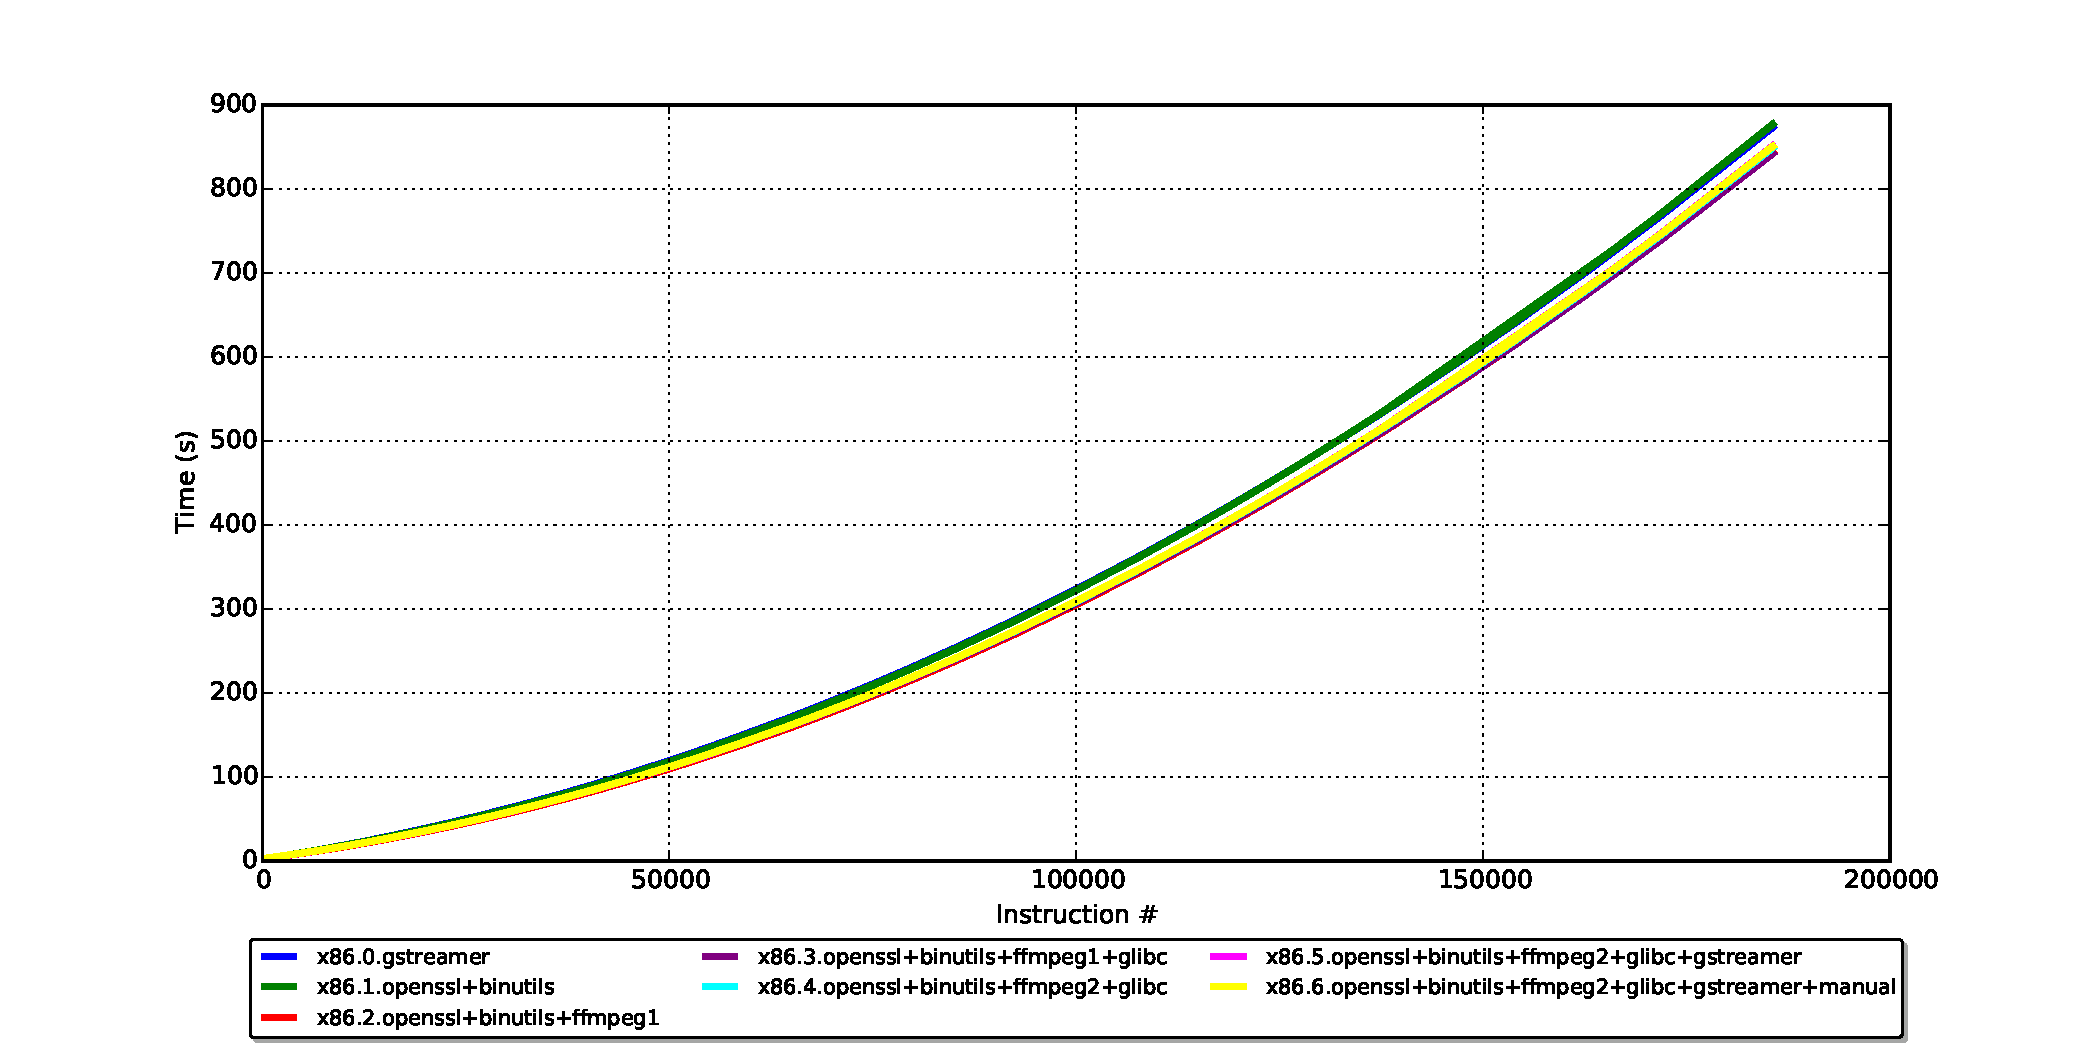
\includegraphics[width=0.8\textwidth]{automata_comparison}%
\caption{Lifting time comparison between different automata.}
\label{fig:automata_time}
\end{figure}

Another important question not answered by the authors in~\cite{Hasabnis2014} is if the automata used impacts the instruction lifting time. Figure~\ref{fig:automata_time} displays the time growth in function of the number of instructions for seven different automata used in my experiments. As the figure shows, up until around 25k instructions, the lifting time difference between automata is negligible. As the number of instructions surpasses 50k, the difference is more clear, although it still is minor. Moreover, there does not seem to exist a relationship between the size of the automata and the lifting time, as the two biggest automata (\textit{x86.5} and \textit{x86.6}) both show smaller growth than the two smallest automata (\textit{x86.0} and \textit{x86.1}). This is a clear upside of bigger automata, since bigger automata tend to have better lifting accuracy, plus the time to create bigger automata is still short.

\section{Supplementary Results}

Alongside with the graphs show, I also provide in the packages detailed results for the lifting runs of each automata, as well as their lifting times. Plus, the graphs containing time growth for the \textit{x86.3} automata, as well as an instruction statistics file for all the binary dumps.


\section{Conclusion} \label{sec:conc}

In this project, I further explored LISC~\cite{Hasabnis2014,LISC}, evaluating it under the \textit{completeness} and \textit{performance} metrics. Considering the completeness methodology presented by Hasabnis and Sekar~\cite{Hasabnis2014}, some changes had to be made in order to reproduce their experiment. Namely, a different set of testing programs and automata were used. Moreover, each test program was evaluated individually, instead of in a bundle. Our results were significantly lower than the reported by the authors, being as high as 7 percentual points for comparable automata and a much smaller set of programs. One possible reason as that in my experiments, duplicate instructions were not eliminated.

The performance experiments have shown a clear discrepancy between the lifting time obtained in my experiments and the one reported in~\cite{Hasabnis2014}. The authors claimed linear complexity for their lifting algorithm, and that the lifting time was of around 8 hours for the whole linux kernel binaries (around 40M instructions). However, in my experiments, I observed a clear quadratic growth of lifting time in function of the binary size, resulting in around 13 hours to lift around 17M instructions. Other experiments also shown how the size of the automata used caused no impact in lifting time.

\bibliographystyle{sbc}
\bibliography{sbc-template}

\end{document}
